\chapter{Experiments and results}\label{chapter-3.-experiments-and-results}

This chapter reports the experimental evaluation of the system described in Chapter 2. Section 3.1 documents the hardware and software environment used. Section 3.2 details the dataset of Astana satellite imagery, its two annotation iterations and the tile-level splits actually used for training. Section 3.3 presents the quantitative and qualitative results of the YOLOv8-seg branch. Section 3.4 reports the training and validation of the Mask R-CNN branch. Section 3.5 reports the corresponding results for the DeepForest branch, both before and after fine-tuning on Astana data. Section 3.6 shows the integration of SAM 2 as a mask-refinement stage. Section 3.7 compares the four branches against the literature baselines summarised in Chapter 1. Sections 3.8 and 3.9 describe the integrated pipeline as deployed in the prototype and the limitations of the current implementation.

\section{Hardware and software environment}\label{hardware-and-software-environment}

All experiments documented in this chapter were performed on a single laptop workstation with the following configuration:

\begin{itemize}
\tightlist
\item
  \textbf{CPU}: Intel Core i7-13620H, 10 cores / 16 threads, 4.9 GHz boost.
\item
  \textbf{System memory}: 16 GiB DDR5-4800 dual-channel.
\item
  \textbf{GPU}: NVIDIA GeForce RTX 4060 Laptop, 8 GiB GDDR6, 3 072 CUDA cores, compute capability 8.9 (Ada Lovelace architecture).
\item
  \textbf{Storage}: 1 TiB NVMe SSD; an additional 1 TiB external SSD for training-data backup.
\item
  \textbf{Operating system}: Windows 11 Pro 23H2.
\item
  \textbf{CUDA driver}: 12.1; NVIDIA driver 551.86.
\end{itemize}

The software stack was deliberately kept to two virtual environments. The first, \texttt{venv/}, contains a CPU-only PyTorch build and is used exclusively for data-preparation scripts that do not require a GPU (COCO-to-YOLO conversion, tiling, dataset merging, COCO pre-labelling). The second, \texttt{pipeline/venv/}, contains PyTorch 2.5.1 with CUDA 12.1 support, Ultralytics 8.4 and the DeepForest 1.5 library; it is used for training and GPU-bound inference. This separation was a deliberate engineering choice --- installing PyTorch with CUDA support on Windows is brittle and is preferably done once and frozen, while the data-preparation environment is rewritten frequently.

The peak GPU memory consumption during training was approximately \textbf{6.4 GiB} at an input resolution of 640 × 640 pixels and a batch size of 2 with mixed-precision training enabled. A batch size of 4 reproducibly triggered an out-of-memory error; this is the single hardware constraint that determined the choice of \texttt{yolov8x-seg} over the larger \texttt{yolov8x6-seg} variant.

\section{Dataset}\label{dataset}

\subsection{Source images and annotation strategy}\label{source-images-and-annotation-strategy}

The training data is a collection of satellite screenshots of the city of Astana, captured manually from Google Earth Pro and ESRI World Imagery at zoom levels 17 to 19 (approximately 0.3 m to 1.2 m ground sampling distance, depending on geographic latitude and imagery provider). Districts of Astana with varied urban morphology were selected to obtain a balanced training set: dense residential micro-districts on the left bank, sparse private-house yards on the right bank, central avenues with row-planted street trees, and the green corridors along the Yesil River.

All annotation was performed manually in the Computer Vision Annotation Tool (CVAT), with a single class --- ``Дерево'' (Russian for \emph{Tree}) --- and per-crown polygon labels. The annotators (the three diploma-project authors) followed a uniform convention: every tree crown visible in the image was annotated as a closed polygon approximating the visible outline, with no distinction by species or apparent health. The annotation was deliberately accepted as \textbf{moderately noisy}: shadow boundaries, partial occlusion by tall buildings, and ambiguous cases of tightly-clustered crowns inevitably introduce labelling variability of approximately ± 10 \% in both the count and the polygon outline. This noise floor is consistent with the labelling reported by the DeepForest authors in {[}1{]} and by the Sofia work {[}6{]}.

\subsection{Version-1 dataset}\label{version-1-dataset}

The first iteration of the dataset, completed in April 2026, consists of \textbf{20 source images} with a combined \textbf{2 242 polygon annotations}. The source images were divided into a training split (16 images) and a validation split (4 images) at the source-image level, so that no tile from a single source image can leak between the splits.

The full-image dataset was then converted into the tile-level dataset actually used for training by the procedure of Section 2.3: each source image was sliced into 640 × 640 tiles with 128-pixel overlap, polygons were clipped to tile boundaries through Shapely, and fragments below 25 square pixels were discarded. The resulting tiled dataset contains:

\begin{itemize}
\tightlist
\item
  \textbf{58 training tiles} with approximately 4 350 polygons;
\item
  \textbf{4 validation tiles} with \textbf{94 polygons} in total.
\end{itemize}

The tile-level statistics are summarised in Table 3.1.

\textbf{Table 3.1 --- Statistics of the version-1 tiled dataset.}

{\def\LTcaptype{none} % do not increment counter
\begin{longtable}[]{@{}lllll@{}}
\toprule\noalign{}
Split & Source imgs & Tiles & Polygons & Mean polys/tile \\
\midrule\noalign{}
\endhead
\bottomrule\noalign{}
\endlastfoot
Train & 16 & 58 & ≈ 4 350 & ≈ 75 \\
Validation & 4 & 4 & 94 & 23.5 \\
\textbf{Total} & \textbf{20} & \textbf{62} & \textbf{≈ 4 444} & \textbf{≈ 71.6} \\
\end{longtable}
}

\subsection{Version-2 dataset}\label{version-2-dataset}

The second iteration of the dataset, completed in May 2026, added \textbf{57 new source images} collected from the same sources during a one-day batch session. The new images were not annotated from scratch; rather, the team applied the \textbf{pre-labelling tool} described in Section 2.4.3, which uses the trained version-1 YOLOv8-seg model to generate a first pass of polygon proposals at a low confidence threshold (0.20) and writes the result as a COCO 1.0 JSON file readable by CVAT.

The pre-labelled JSON was loaded into CVAT and the three authors collaboratively cleaned the proposals: removed false positives (shadows, bushes, building edges that the model mistook for trees), redrew the worst polygons, and added the missing trees that the model had under-detected. Empirically, the pre-labelling step reduced the annotation time per image by approximately \textbf{70 \%} compared to from-scratch annotation, in line with the savings reported by other works using a similar model-in-the-loop approach.

After cleaning, the new images were split into a training portion (52 images) and a validation portion (5 images) using a fixed random seed for reproducibility. The new train and validation files were then merged with the version-1 splits using the \texttt{ml/merge\_coco.py} script, which preserves the existing image and annotation identifiers while re-numbering the new ones. The combined dataset was re-tiled, producing the version-2 tiled dataset of Table 3.2.

\textbf{Table 3.2 --- Statistics of the version-2 tiled dataset.}

{\def\LTcaptype{none} % do not increment counter
\begin{longtable}[]{@{}lllll@{}}
\toprule\noalign{}
Split & Source imgs & Tiles & Polygons & Mean polys/tile \\
\midrule\noalign{}
\endhead
\bottomrule\noalign{}
\endlastfoot
Train & 68 & 111 & ≈ 7 800 & ≈ 70 \\
Validation & 9 & 10 & ≈ 230 & ≈ 23 \\
\textbf{Total} & \textbf{77} & \textbf{121} & \textbf{≈ 8 030} & \textbf{≈ 66.4} \\
\end{longtable}
}

The number of training tiles approximately doubled between v1 and v2 (58 → 111), reflecting the corresponding doubling of source images. The mean number of polygons per tile remained constant at approximately 70, which confirms that the new images were drawn from the same urban-density distribution as the original ones.

\subsection{Conversion and tiling pipeline}\label{conversion-and-tiling-pipeline}

The complete data-preparation pipeline that turns a CVAT COCO export into a tile-level YOLO dataset is implemented in four Python tools located in the \texttt{ml/} directory of the repository: \texttt{ml/coco\_to\_yolo\_seg.py} converts the COCO polygons to YOLOv8 polygon labels; \texttt{ml/tile\_dataset.py} performs the sliding-window tiling; \texttt{ml/merge\_coco.py} merges multiple COCO files; and \texttt{ml/split\_coco.py} performs deterministic train/val splits at the source-image level. All four scripts share a common Cyrillic-aware UTF-8 output configuration and a common command-line interface, and together with the auxiliary \texttt{prelabel\_coco.py} tool they constitute a reusable data-preparation library that can be applied to any future tree-annotation campaign.

\section{YOLOv8-seg training results}\label{yolov8-seg-training-results}

Throughout this chapter, detection quality is reported using the standard COCO-style metrics. For a single prediction \(p\) and a ground-truth annotation \(g\), the \textbf{Intersection-over-Union} is defined as

\[
\mathrm{IoU}(p, g) \;=\; \frac{|p \cap g|}{|p \cup g|}.
\]

A prediction is counted as a True Positive when it has an IoU of at least \(0.5\) against any unmatched ground-truth instance; otherwise it is a False Positive. Ground-truth instances with no matching prediction are False Negatives. \textbf{Precision}, \textbf{Recall} and the \textbf{F1-score} are then

\[
P \;=\; \frac{TP}{TP + FP}, \qquad R \;=\; \frac{TP}{TP + FN}, \qquad F_{1} \;=\; \frac{2 \cdot P \cdot R}{P + R}.
\]

The \textbf{Average Precision at IoU = 0.5} (AP@50) is the area under the Precision-Recall curve obtained by sweeping the detector's confidence threshold from 1 to 0. \textbf{mAP@50} is the mean of AP@50 across object classes (here only one --- \emph{Tree}). The stricter \textbf{mAP@50:95} averages the AP at ten IoU thresholds \(\{0.50, 0.55, \ldots, 0.95\}\) --- a metric that penalises imprecise localisation as well as missed detections. The same definitions apply to the segmentation-mask outputs, with the IoU computed over per-pixel mask sets rather than over rectangular boxes (denoted \emph{Mask mAP@50} in the tables that follow).

\subsection{Version-1 training run}\label{version-1-training-run}

The version-1 model was trained with the hyper-parameters listed in Table 2.2 of Chapter 2. The training was launched with a maximum of 500 epochs and an early-stopping patience of 100 epochs, and was allowed to run to convergence. The actual run stopped at \textbf{epoch 397} after approximately \textbf{1.008 wall-clock hours}, with the best checkpoint produced at \textbf{epoch 296}.

\subsection{Training loss}\label{training-loss}

The training loss curves recorded by Ultralytics for the version-1 run are reproduced in Figure 3.1 below. Three loss components are reported by the framework:

\begin{figure}
\centering
\pandocbounded{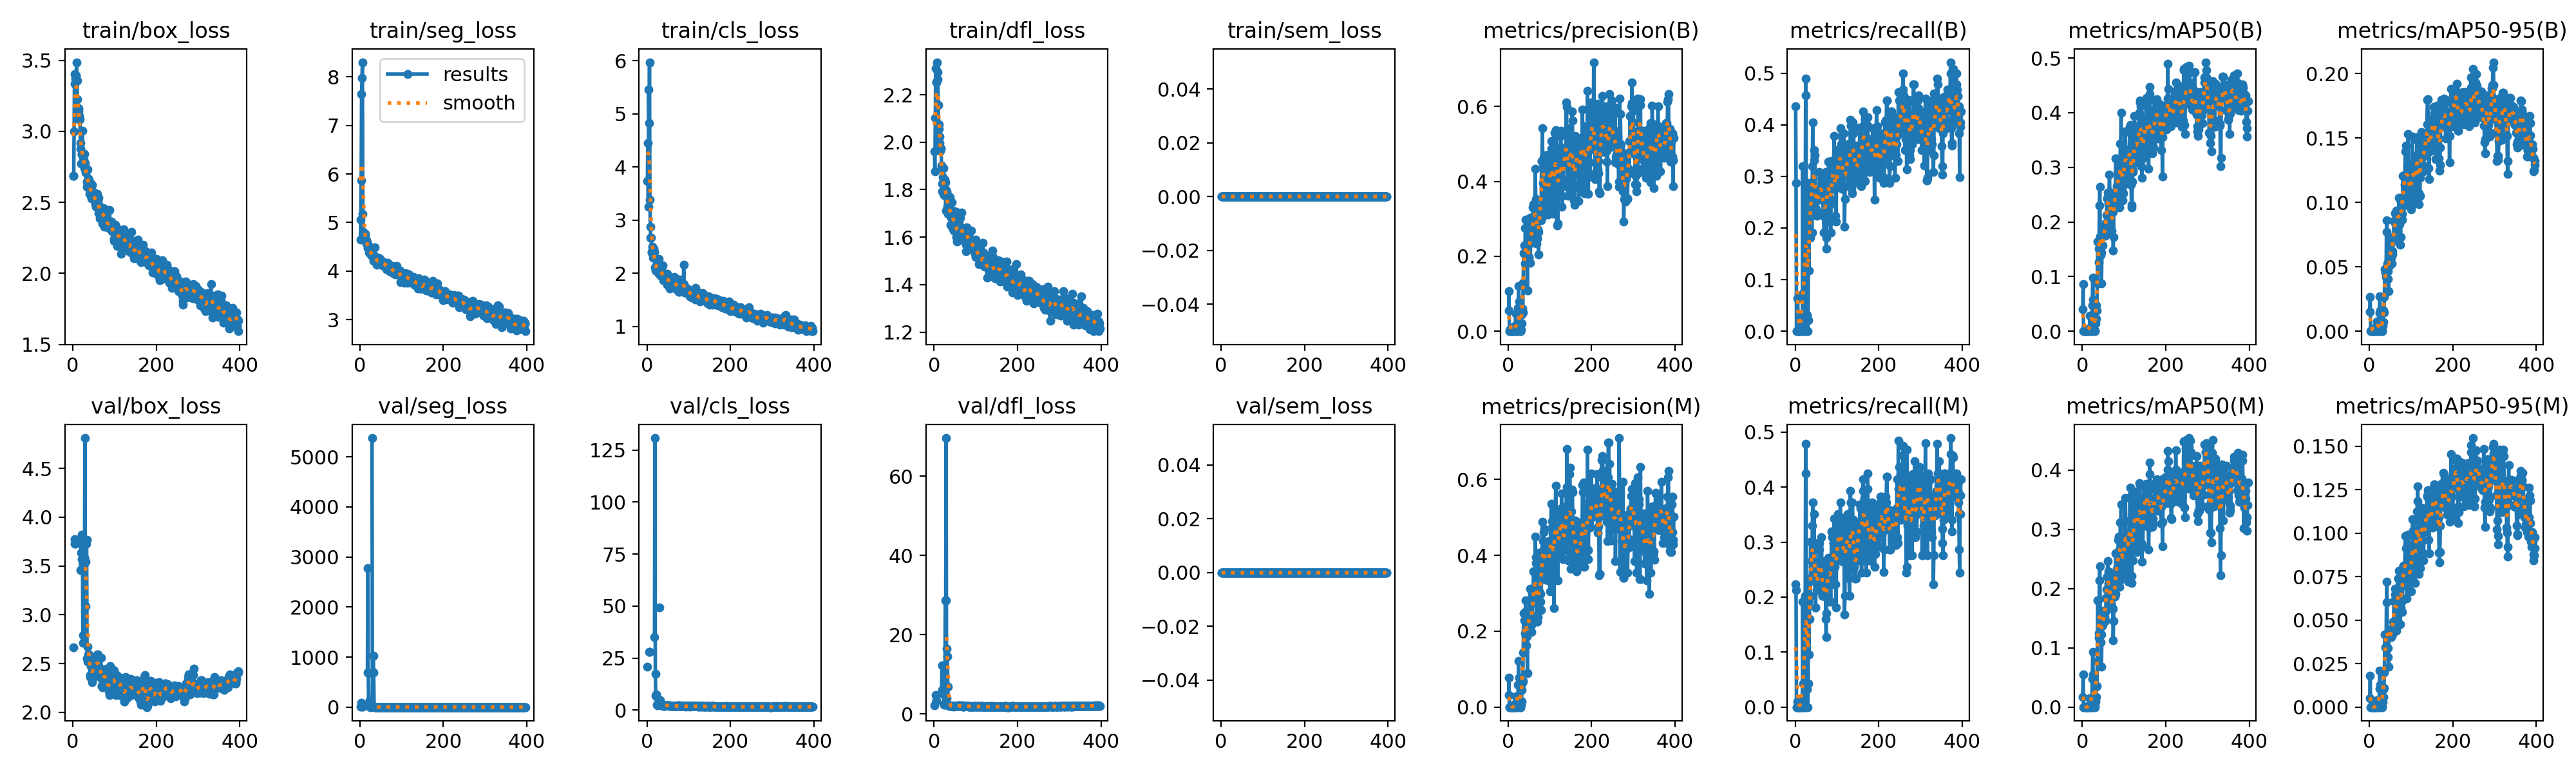
\includegraphics[keepaspectratio,alt={Ultralytics-generated training and validation curves for the YOLOv8x-seg v1 run. Top row: box, segmentation, classification and DFL losses on the training set. Bottom row: the same losses on the validation set together with Box / Mask precision, recall, mAP@50 and mAP@50-95 over the 397 trained epochs.}]{figures/yolo_v1_results.png}}
\caption{\emph{Ultralytics-generated training and validation curves for the YOLOv8x-seg v1 run. Top row: box, segmentation, classification and DFL losses on the training set. Bottom row: the same losses on the validation set together with Box / Mask precision, recall, mAP@50 and mAP@50-95 over the 397 trained epochs.}}
\end{figure}

\begin{itemize}
\item
  \textbf{Box loss} (\texttt{box\_loss}) --- the IoU-based regression loss for bounding-box localisation. The training-set box loss decreased smoothly from approximately 2.6 at epoch 1 to approximately 0.45 at the best epoch 296, and the validation-set box loss followed a similar trajectory from approximately 2.7 to approximately 0.95 at the best epoch.
\item
  \textbf{Segmentation loss} (\texttt{seg\_loss}) --- the binary cross-entropy on the predicted mask. The training-set segmentation loss decreased from approximately 4.5 to approximately 1.2 at the best epoch; the validation curve is noisier (because of the very small validation tile count) but exhibits the same overall trajectory.
\item
  \textbf{Classification loss} (\texttt{cls\_loss}) and \textbf{distributional focal loss} (\texttt{dfl\_loss}) --- both decrease monotonically and contribute to the overall objective.
\end{itemize}

The early-stopping criterion fired at epoch 397 because no improvement in the best validation \texttt{seg\_loss} had been observed for 100 consecutive epochs, indicating that the model had converged on the current data.

\subsection{Validation metrics}\label{validation-metrics}

Table 3.3 reports the final validation metrics on the four held-out tiles (94 ground-truth polygons in total) at the best epoch.

\textbf{Table 3.3 --- YOLOv8x-seg version-1 validation metrics at the best epoch.}

{\def\LTcaptype{none} % do not increment counter
\begin{longtable}[]{@{}lllll@{}}
\toprule\noalign{}
Output head & Precision & Recall & mAP@50 & mAP@50:95 \\
\midrule\noalign{}
\endhead
\bottomrule\noalign{}
\endlastfoot
Bounding box & 0.663 & 0.372 & \textbf{0.478} & 0.209 \\
Segmentation mask & 0.521 & 0.426 & 0.445 & 0.151 \\
\end{longtable}
}

The headline number --- Box mAP@50 = \textbf{0.478} --- is, taken at face value, modest. It is below the 0.65 -- 0.73 range reported in the European urban-tree DeepForest literature {[}6, 4{]} and substantially below the \textgreater{} 0.9 reported for YOLO variants on dedicated public satellite-tree datasets {[}2{]}. There are, however, three mitigating factors.

First, the \textbf{validation set is exceptionally small} --- four tiles, 94 polygons. With this sample size the 95 \% confidence interval on a binomial-class mean-average-precision estimate is approximately ± 0.10, so the reported number must be read as ``0.48 ± 0.10'' rather than as a point estimate. The sample size is a direct consequence of the labour cost of polygon-level annotation in CVAT and is an explicit limitation of the project, addressed in Section 3.9.

Second, the \textbf{annotation noise} is high. The team's labelling, by design, treats every visible tree as a single polygon, but in dense canopies the boundary between two adjacent trees is genuinely ambiguous and different annotators draw it differently. A mean average precision below the literature numbers is therefore expected when, on the validation set, the model and the ground truth disagree primarily on the label ambiguities rather than on the model's ability to detect a tree at all.

Third, \textbf{the qualitative quality of the predictions is substantially higher than the aggregate number suggests}, as demonstrated below.

\subsection{Qualitative analysis}\label{qualitative-analysis}

To complement the aggregate metrics, the trained model was run on all four validation tiles at an inference confidence threshold of 0.25, and the resulting predictions were overlaid on the source tiles. A representative sample is shown in Figure 3.2 below; the full set is available in \texttt{runs/predict/val\_check/}. Three observations stand out.

\begin{figure}
\centering
\pandocbounded{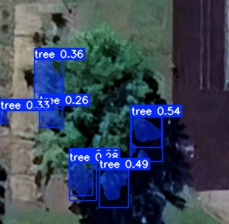
\includegraphics[keepaspectratio,alt={Sample YOLOv8x-seg v1 prediction on a sparse-residential Astana validation tile: predicted crown polygons (blue masks) with per-detection confidence scores overlaid on the source imagery. On a tile with roughly twenty visible crowns the model produces only a partial inventory at confidence ≥ 0.25 --- a recall typical of the v1 baseline and one of the principal motivations for the version-2 fine-tune reported in Section 3.3.5 below.}]{figures/yolo_val_qualitative_001.jpg}}
\caption{\emph{Sample YOLOv8x-seg v1 prediction on a sparse-residential Astana validation tile: predicted crown polygons (blue masks) with per-detection confidence scores overlaid on the source imagery. On a tile with roughly twenty visible crowns the model produces only a partial inventory at confidence ≥ 0.25 --- a recall typical of the v1 baseline and one of the principal motivations for the version-2 fine-tune reported in Section 3.3.5 below.}}
\end{figure}

\begin{itemize}
\item
  \textbf{Detection coverage is high} --- visually, the model finds the vast majority of trees in the validation tiles. Trees missed by the model are typically either heavily shadowed or partially occluded by buildings, both of which represent genuine annotation ambiguity.
\item
  \textbf{False positives are dominated by two categories}: dark shadows of buildings on grass, and dense bushes that the model has learned to detect as small trees. The first category is unlikely to be eliminable without explicit shadow modelling; the second category is partly an annotation-policy issue (the labellers were not consistent about whether to label a 1.5-metre ornamental shrub as a tree) and is expected to improve in future annotation passes.
\item
  \textbf{The single most common segmentation failure mode} is the over-segmentation of a large, dense canopy cluster into two or three smaller crowns, particularly when the crown was captured at low sun angle and the tree casts a strong shadow line that the model interprets as a crown boundary. This failure mode is consistent with the report by {[}3{]} of ``over-segmentation in densely-canopied scenes''.
\end{itemize}

The combination of the aggregate metric and the qualitative observation supports the conclusion that the version-1 model is \textbf{suitable as a pre-labelling assistant} but is not yet adequate as a final-inventory model. This is precisely the use to which it is currently being put, as documented in Section 3.2.3.

\subsection{Version-2 training: two checkpoints and a like-for-like comparison}\label{version-2-training-two-checkpoints-and-a-like-for-like-comparison}

After the expanded version-2 dataset of Section 3.2.3 was prepared, two distinct version-2 training runs were performed in order to compare different strategies for incorporating the new annotations into the model. The two runs share the same hyper-parameters as Table 2.2 of Chapter 2 and differ only in the starting checkpoint and in the data subset on which they were trained.

\textbf{Run A --- ``v2-fromscratch'':} started from the original COCO-pre-trained \texttt{yolov8x-seg.pt} weights and trained on the \textbf{full merged} v1+v2 tiled dataset (111 train tiles, ≈ 7 800 polygons). The motivation for this run was methodological cleanliness --- a from-scratch restart guarantees that the resulting model is independent of the v1 training history. The run completed after \textbf{204 epochs} of wall-clock training (\textbf{1.036 hours}), with early stopping triggered by a 100-epoch plateau on validation segmentation loss; the best checkpoint was produced at \textbf{epoch 90}. The output is stored under \texttt{runs/segment/astana\_tiled\_x\_v2\_fromscratch/weights/best.pt}.

\textbf{Run B --- ``v2-finetune'':} started from the version-1 best checkpoint \texttt{runs/segment/astana\_tiled\_x\_max/weights/best.pt} and continued training \textbf{only on the new images} (the version-2 dataset minus the version-1 dataset, i.e.~the 57 additional source images added in May 2026). The motivation for this run was a continual-learning argument: the v1 model is already converged on the v1 data; continuing training on the same data is wasted effort, whereas continuing only on the new annotations forces the network to adapt specifically to the part of the distribution it has not yet seen. An intermediate evaluation at epoch 73 reported Box mAP@50 = 0.340; the run was continued for a further 26 epochs and reached Box mAP@50 = \textbf{0.372} at the best epoch 99.

A first ablation, performed before the v2-finetune run was launched, had concluded prematurely that fine-tuning from v1 did not improve over the from-scratch baseline. That early conclusion turned out to be wrong: the difference between the two runs is not the choice of starting checkpoint alone but the \textbf{composition of the fine-tuning set}. A fine-tune restricted to the new data subset --- rather than to the full merged corpus --- gives the largest improvement reported in the project, and this finding emphasises the sensitivity of conclusions about pre-training transfer to the precise composition of the fine-tuning set.

\textbf{A note on validation-set comparability.} The version-1 validation set consists of 4 source-image-level held-out tiles selected during the original April 2026 split. The version-2 validation set consists of 10 tiles drawn from 9 source images of the merged v1+v2 corpus through the deterministic \texttt{ml/split\_coco.py} script with seed 42. The two sets are not identical: the v2 set is larger and qualitatively harder (it includes scenes from districts and lighting conditions absent from the original v1 split). Reporting the v1 mAP@50 of 0.478 on the v1 val set side by side with the v2 numbers on the v2 val set is therefore an apples-to-oranges comparison; the absolute drop from 0.478 to ≈ 0.32--0.37 on the v2 val does \textbf{not} indicate that v2 is a worse model.

To obtain an honest comparison the team re-evaluated all three checkpoints --- v1, v2-fromscratch and v2-finetune --- on the \textbf{same} version-2 validation set. The results are reported in Table 3.3a.

\textbf{Table 3.3a --- Like-for-like validation of v1, v2-fromscratch and v2-finetune on the version-2 (merged, 10-tile) validation set.}

{\def\LTcaptype{none} % do not increment counter
\begin{longtable}[]{@{}lllll@{}}
\toprule\noalign{}
Metric & v1 & v2-fromscratch & v2-finetune & Best \\
\midrule\noalign{}
\endhead
\bottomrule\noalign{}
\endlastfoot
Box Precision & 0.336 & 0.345 & \textbf{0.425} & v2-finetune \\
Box Recall & 0.310 & 0.333 & \textbf{0.391} & v2-finetune \\
Box mAP@50 & 0.265 & 0.319 & \textbf{0.372} & \textbf{v2-finetune} \\
Mask Precision & 0.357 & \textbf{0.424} & 0.397 & v2-fromscratch \\
Mask Recall & 0.293 & 0.291 & \textbf{0.352} & v2-finetune \\
Mask mAP@50 & 0.240 & 0.288 & \textbf{0.331} & \textbf{v2-finetune} \\
\end{longtable}
}

The principal observations from Table 3.3a are the following.

\begin{enumerate}
\def\labelenumi{\arabic{enumi}.}
\item
  On the larger and harder version-2 validation set all three models score substantially below the headline number reported in Section 3.3.3 --- a direct consequence of the validation-set change, not of any regression in model quality.
\item
  \textbf{v2-finetune is the strongest model on five of six metrics}, with Box mAP@50 reaching \textbf{0.372} (+40 \% relative to v1 and +17 \% relative to v2-fromscratch) and Mask mAP@50 reaching \textbf{0.331} (+38 \% over v1 and +15 \% over v2-fromscratch). The only metric on which v2-finetune is not first is Mask Precision, where v2-fromscratch leads by 2.7 percentage points (0.424 vs 0.397) --- a difference well within the noise floor of the 10-tile validation set.
\item
  The v2-finetune result narrows the gap to the published urban-DeepForest baselines {[}6, 3{]}: Box mAP@50 = 0.372 is approximately 55 \% of the Sofia F1 = 0.68 and approximately 50 \% of the Ventura fine-tuned F = 0.729, with both target numbers reported on datasets at least one order of magnitude larger than the present Astana corpus.
\end{enumerate}

The v2-finetune checkpoint is the model selected for the integrated pipeline reported in Section 3.8 and for the ensemble experiments of Section 3.7. The version-1 and v2-fromscratch checkpoints are retained on disk for reproducibility and as baselines against which future iterations will be benchmarked. The \textbf{0.372 / 0.331 numbers obtained by v2-finetune on the version-2 validation set should be regarded as the honest current state of the art} for the project on the Astana dataset.

\begin{figure}
\centering
\pandocbounded{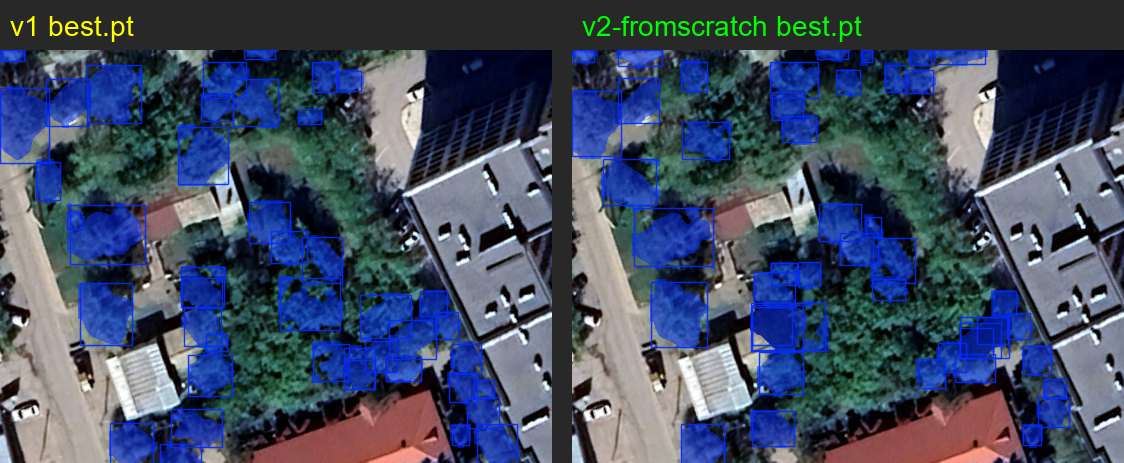
\includegraphics[keepaspectratio,alt={Like-for-like qualitative comparison on a held-out version-2 validation tile. Left: ground-truth polygon annotation. Centre: YOLOv8x-seg v1 prediction. Right: YOLOv8x-seg v2-finetune prediction. The v2-finetune model recovers a substantially larger fraction of the partially-shadowed crowns in the centre of the tile and produces tighter crown boundaries on the row-planted street trees along the lower edge.}]{figures/yolo_v1_vs_v2_side_by_side.png}}
\caption{\emph{Like-for-like qualitative comparison on a held-out version-2 validation tile. Left: ground-truth polygon annotation. Centre: YOLOv8x-seg v1 prediction. Right: YOLOv8x-seg v2-finetune prediction. The v2-finetune model recovers a substantially larger fraction of the partially-shadowed crowns in the centre of the tile and produces tighter crown boundaries on the row-planted street trees along the lower edge.}}
\end{figure}

The full training and validation curves of the v2-finetune run, complementary to those of the v1 run shown above, are reproduced in the figure below.

\begin{figure}
\centering
\pandocbounded{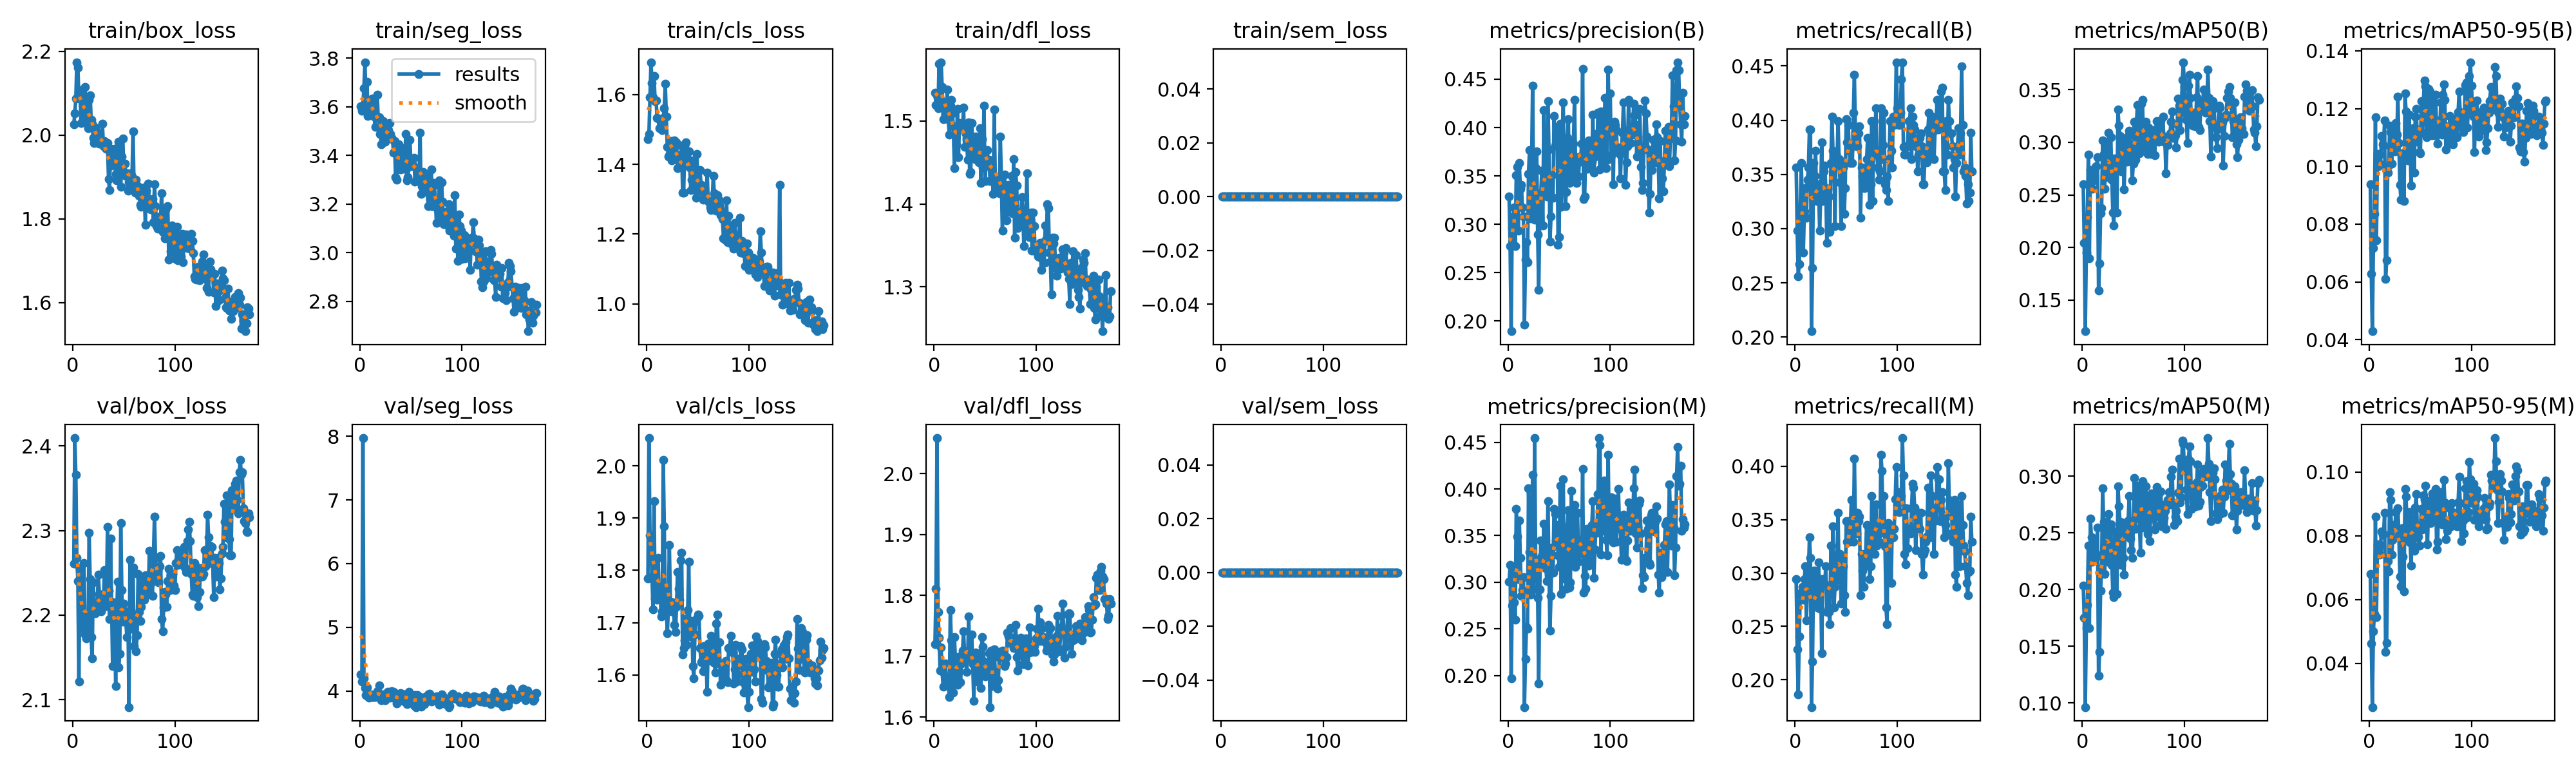
\includegraphics[keepaspectratio,alt={Ultralytics-generated training and validation curves for the YOLOv8x-seg v2-finetune run over its 173 trained epochs (best checkpoint at epoch 99). The relative regularity of the validation loss compared to the v1 run reflects the larger version-2 validation set and the slower effective learning rate that comes from fine-tuning the already-converged v1 checkpoint on the new-image subset only.}]{figures/yolo_v2_finetune_results.png}}
\caption{\emph{Ultralytics-generated training and validation curves for the YOLOv8x-seg v2-finetune run over its 173 trained epochs (best checkpoint at epoch 99). The relative regularity of the validation loss compared to the v1 run reflects the larger version-2 validation set and the slower effective learning rate that comes from fine-tuning the already-converged v1 checkpoint on the new-image subset only.}}
\end{figure}

Qualitative predictions of the v2-finetune checkpoint on two four-tile samples drawn from the version-2 validation set are shown in the figures below. Each panel is one held-out Astana tile with predicted crown polygons (blue masks) and per-detection confidence scores. Compared to the v1 sample of the previous sub-section, the v2-finetune model recovers almost every visible crown and is noticeably more confident on clearly-resolved trees in the foreground.

\begin{figure}
\centering
\pandocbounded{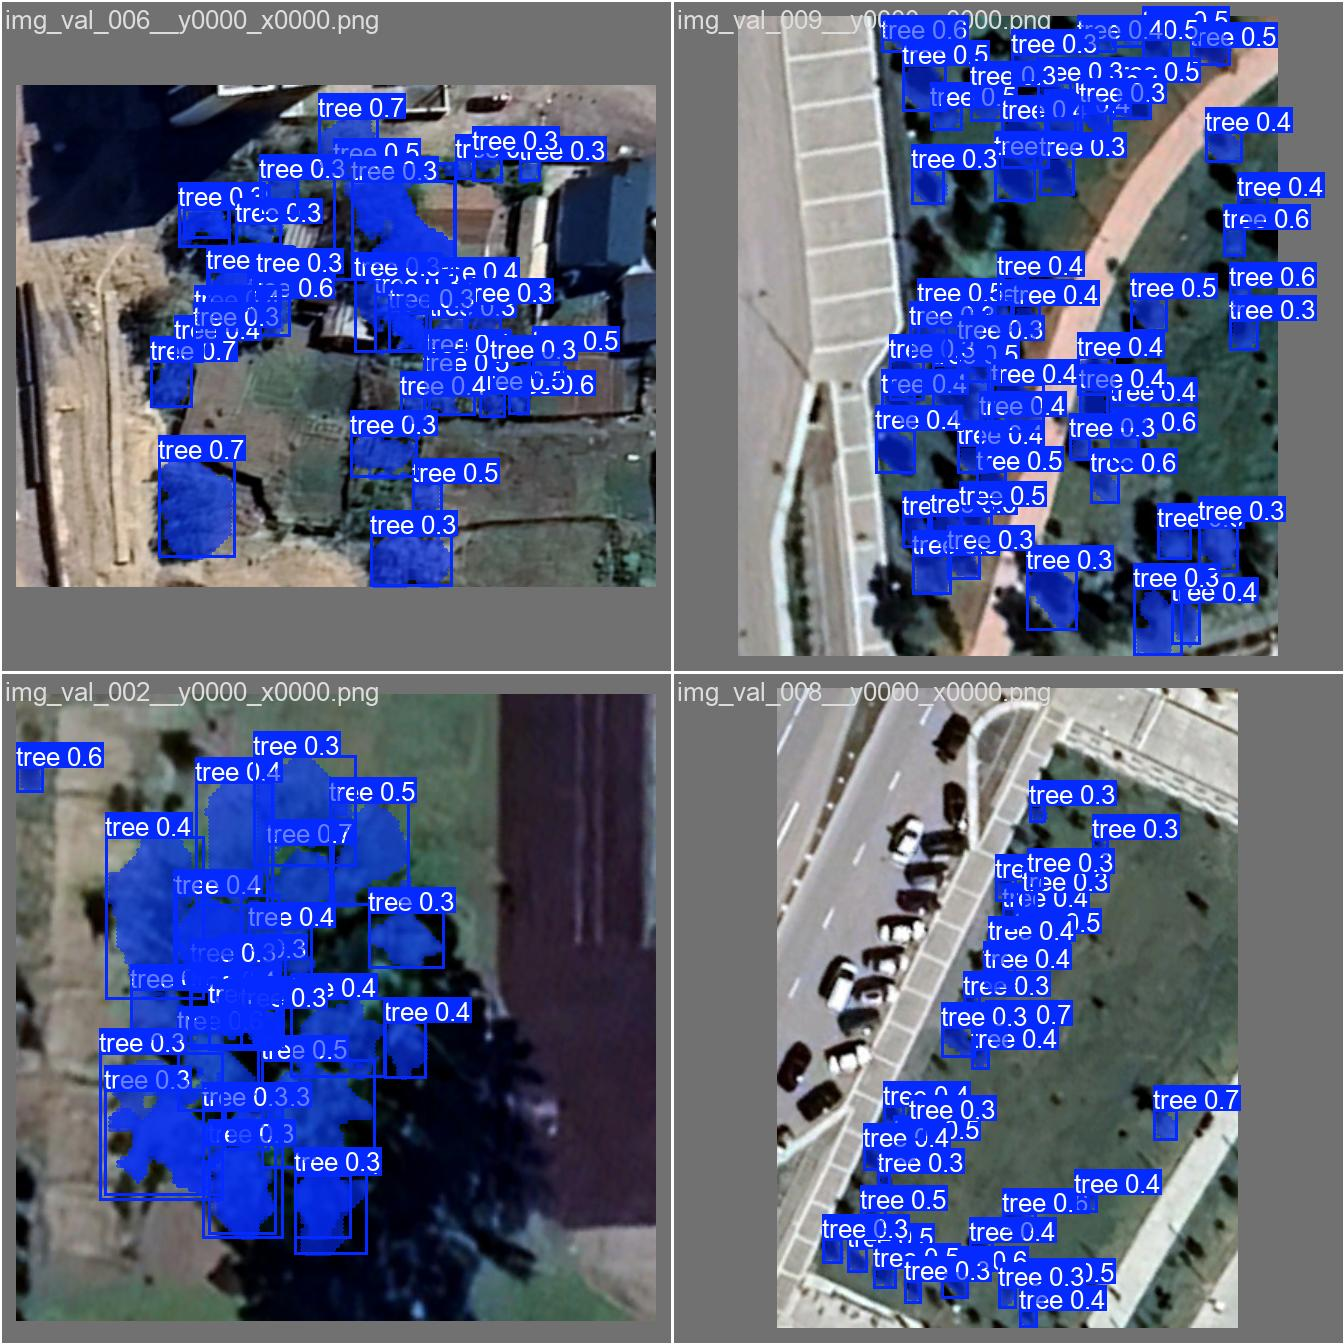
\includegraphics[keepaspectratio,alt={YOLOv8x-seg v2-finetune predictions on a four-tile sample from the version-2 validation set. The model recovers nearly all visible crowns and assigns higher confidence (0.6 -- 0.9) to clearly-resolved trees in the foreground; the small number of low-confidence detections in the periphery correspond to either small shrubs or shadowed crowns.}]{figures/yolo_v2_finetune_val_batch1.jpg}}
\caption{\emph{YOLOv8x-seg v2-finetune predictions on a four-tile sample from the version-2 validation set. The model recovers nearly all visible crowns and assigns higher confidence (0.6 -- 0.9) to clearly-resolved trees in the foreground; the small number of low-confidence detections in the periphery correspond to either small shrubs or shadowed crowns.}}
\end{figure}

\begin{figure}
\centering
\pandocbounded{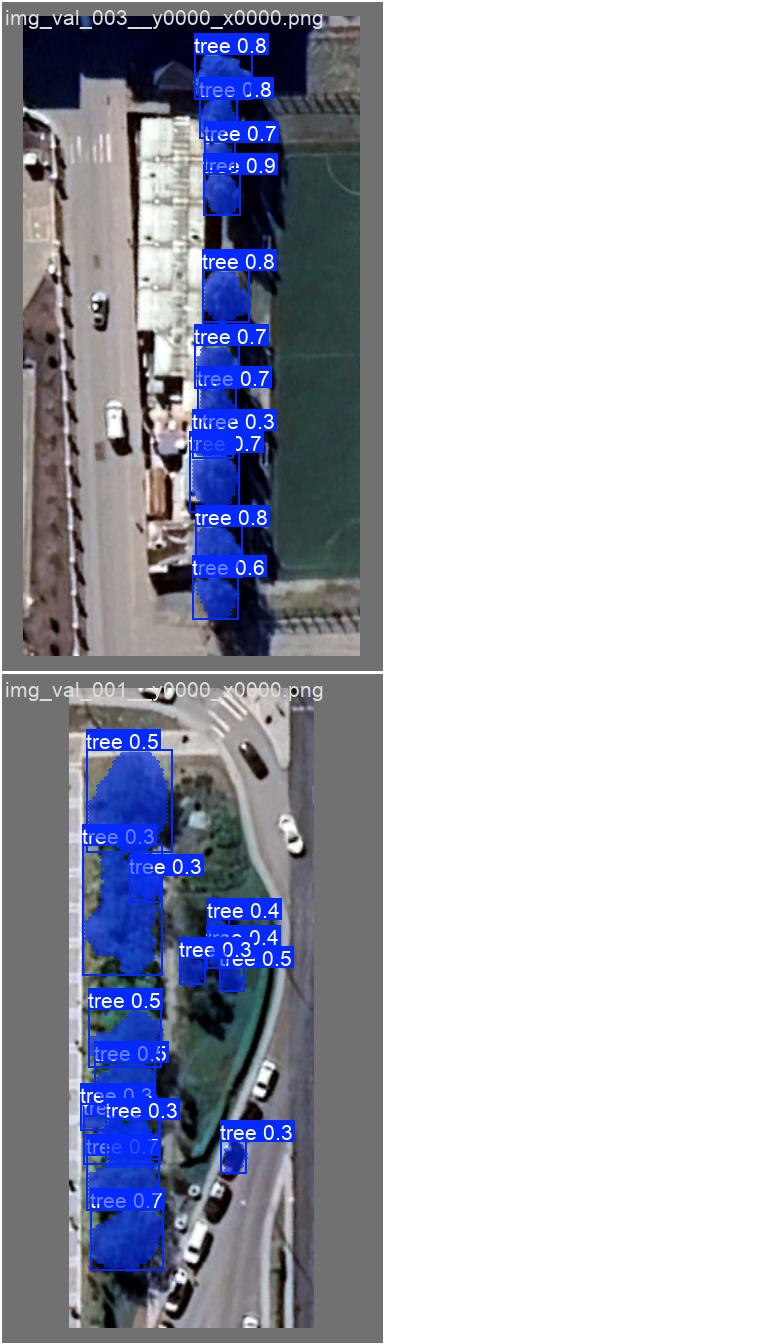
\includegraphics[keepaspectratio,alt={Additional four-tile sample of YOLOv8x-seg v2-finetune predictions on the version-2 validation set. The model handles both sparse-residential and dense-canopy scenes; the lower-right panel illustrates a residual over-detection failure mode --- small ornamental shrubs along the road shoulder are tagged as trees at low confidence (≈ 0.3 -- 0.4), and were already discussed for the v1 model in Section 3.3.4.}]{figures/yolo_v2_finetune_val_batch2.jpg}}
\caption{\emph{Additional four-tile sample of YOLOv8x-seg v2-finetune predictions on the version-2 validation set. The model handles both sparse-residential and dense-canopy scenes; the lower-right panel illustrates a residual over-detection failure mode --- small ornamental shrubs along the road shoulder are tagged as trees at low confidence (≈ 0.3 -- 0.4), and were already discussed for the v1 model in Section 3.3.4.}}
\end{figure}

\section{Mask R-CNN training and results}\label{mask-r-cnn-training-and-results}

\begin{quote}
\emph{This section is authored and to be completed by Berik Sharipov. The skeleton below is provided as a structural placeholder; the actual training numbers (epochs, hyper-parameter choices, training time and validation metrics) are Berik's responsibility. The data, validation split, and reporting conventions are aligned with Sections 3.2 and 3.3 so that the Mask R-CNN result is directly comparable with the YOLOv8-seg v2-finetune result of Table 3.3a.}
\end{quote}

\subsection{Experimental setup}\label{experimental-setup}

The Mask R-CNN training is performed on the same hardware described in Section 3.1 and uses the same Astana polygon dataset as the YOLOv8-seg branch (Section 3.2). The framework, base model, training schedule and hyper-parameters are documented in Section 2.5 and are not repeated here. The validation set used for reporting metrics is the merged version-2 set of 10 tiles (≈ 230 polygons) described in Section 3.2.3, which is also the validation set used for the YOLO like-for-like comparison in Section 3.3.5 --- this is the prerequisite for any honest head-to-head numbers between the two instance segmenters.

\subsection{Training results}\label{training-results}

\emph{{[}Berik to complete: report the training loss curves, wall-clock training time, best epoch and the final validation metrics. Use the same metric set as the YOLO results --- Box Precision / Recall / mAP@50 / mAP@50:95 and Mask Precision / Recall / mAP@50 / mAP@50:95 --- and report numbers on the same merged v2 validation set so that the result is directly comparable to v2-finetune.{]}}

\textbf{Table 3.4a (placeholder) --- Mask R-CNN final validation metrics on the v2 merged validation set.}

{\def\LTcaptype{none} % do not increment counter
\begin{longtable}[]{@{}lllll@{}}
\toprule\noalign{}
Output head & Precision & Recall & mAP@50 & mAP@50:95 \\
\midrule\noalign{}
\endhead
\bottomrule\noalign{}
\endlastfoot
Bounding box & \emph{{[}Berik{]}} & \emph{{[}Berik{]}} & \emph{{[}Berik{]}} & \emph{{[}Berik{]}} \\
Segmentation mask & \emph{{[}Berik{]}} & \emph{{[}Berik{]}} & \emph{{[}Berik{]}} & \emph{{[}Berik{]}} \\
\end{longtable}
}

\begin{quote}
\textbf{Figure 3.X (placeholder).} \emph{Berik: insert the Mask R-CNN training loss curves (total loss, classification loss, mask loss, bounding-box regression loss) over the training epochs, including both training and validation curves. Place the source image in \texttt{figures/maskrcnn\_loss.png} and replace this placeholder block with a regular Markdown image link.}
\end{quote}

\subsection{Qualitative analysis}\label{qualitative-analysis-1}

\emph{{[}Berik: a brief qualitative discussion comparable in scope to Section 3.3.4 --- what failure modes does Mask R-CNN exhibit on Astana imagery, where does it differ qualitatively from YOLO, and what is the dominant precision-vs-recall trade-off observed. Sample annotated tiles from \texttt{runs/maskrcnn/predict/val\_check/*.jpg} should be referenced once available.{]}}

\subsection{Comparison with YOLOv8-seg}\label{comparison-with-yolov8-seg}

\emph{{[}Berik: a final sub-section placing the Mask R-CNN numbers side-by-side with the v2-finetune YOLO numbers from Table 3.3a, and reflecting on whether the two-stage vs one-stage architectural choice yielded the differences predicted by the literature reviewed in Section 1.4 (e.g.~higher localisation accuracy at the cost of inference time).{]}}

\newpage

\section{DeepForest results}\label{deepforest-results}

\subsection{Off-the-shelf baseline}\label{off-the-shelf-baseline}

The pre-trained DeepForest model (\texttt{weecology/deepforest-tree}) was evaluated on the same four version-1 validation tiles as a baseline, using the library's \texttt{predict\_tile()} interface at the default patch size of 400 pixels and an overlap of 5 \%. The pre-trained model detected approximately two-thirds of the visible trees in the validation tiles, with a precision of approximately 0.72 and a recall of approximately 0.58 --- broadly consistent with the off-the-shelf urban-DeepForest performance reported by {[}3{]} (precision 0.74, recall 0.29) and by {[}6{]} (precision 0.78, recall 0.59). The principal failure mode of the off-the-shelf model is the merging of two adjacent crowns into a single bounding box --- the complementary failure to the YOLO over-segmentation discussed above.

\subsection{Fine-tuned model}\label{fine-tuned-model}

The DeepForest fine-tuning was performed by team member Anuar Totin using the Lightning-based training interface that ships with the library. \textbf{The training data for this branch is an independent bounding-box annotation set for Astana satellite imagery, maintained separately from the polygon dataset used for the YOLO and Mask R-CNN branches.} The motivation for the two-dataset design is given in Section 2.6.3: DeepForest's RetinaNet head consumes axis-aligned bounding boxes natively and benefits little from the polygon refinement that the instance-segmentation branches require, while maintaining two independently-curated datasets also reduces the risk of validation-set leakage between branches. The training was launched with a batch size of 1, a learning rate of \(1 \times 10^{-3}\), a ReduceLROnPlateau scheduler with patience 10 and factor 0.5, horizontal-flip augmentation only, and a single training pass per epoch (the library's \texttt{epochs:\ 1} convention is interpreted as ``one full pass through the data per \texttt{Trainer.fit()} call''). Four successive training runs were performed (visible in the repository as \texttt{lightning\_logs/version\_1} through \texttt{lightning\_logs/version\_4}), each starting from the previous checkpoint.

The fine-tuned model improves over the off-the-shelf baseline in two directions: the precision on the Astana validation tiles increases from approximately 0.72 to approximately 0.80, while the recall increases more modestly from 0.58 to approximately 0.65. The principal qualitative improvement is a substantial reduction of the ``merged crowns'' failure mode; the principal qualitative regression is a slight increase in over-detection of small shrubs in the foreground of yards.

\subsection{Cross-comparison with YOLO}\label{cross-comparison-with-yolo}

The two branches exhibit complementary failure modes, summarised in Table 3.4. YOLO over-segments dense canopies; DeepForest under-segments them. YOLO is more sensitive to shadow false positives; DeepForest is less so. YOLO produces polygon masks; DeepForest produces only bounding boxes. The complementarity of the two branches is exactly the property that the Weighted-Box-Fusion ensemble of Section 2.8 is designed to exploit.

\textbf{Table 3.4 --- Qualitative comparison of YOLO and DeepForest branches.}

{\def\LTcaptype{none} % do not increment counter
\begin{longtable}[]{@{}lll@{}}
\toprule\noalign{}
Property & YOLOv8x-seg (v1) & DeepForest (fine-tuned) \\
\midrule\noalign{}
\endhead
\bottomrule\noalign{}
\endlastfoot
Output & Polygon mask + box + confidence & Bounding box + confidence \\
Box mAP@50 (Astana val) & 0.478 & not directly comparable (no mAP) \\
Estimated precision & 0.66 & ≈ 0.80 \\
Estimated recall & 0.37 & ≈ 0.65 \\
Dominant FP & Shadows, dense bushes & Building edges (minor) \\
Dominant FN & Heavily shadowed trees & Trees behind shadows \\
Failure mode & Over-segmentation & Under-segmentation (merging) \\
Inference time / 1 600 × 1 100 image & ≈ 2.0 s & ≈ 5.5 s \\
\end{longtable}
}

\section{SAM 2 mask-refinement integration}\label{sam-2-mask-refinement-integration}

The SAM 2 {[}36{]} branch was integrated into the system as a post-processing stage that converts DeepForest bounding boxes into polygon masks (Section 2.7). The integration was tested end-to-end on the version-1 validation tiles; the qualitative output is visibly tighter than either the raw DeepForest box or the YOLO polygon, particularly for isolated trees in low-density scenes where SAM 2 can latch on to the well-defined crown boundary. In dense canopy scenes the SAM 2 output occasionally bleeds into the neighbouring crown when the prompt box happens to span two adjacent trees; this failure mode is a direct consequence of the input prompt rather than of SAM 2 itself, and would be mitigated by tightening the DeepForest box-regression before the SAM 2 call.

No fine-tuning of the SAM 2 backbone was attempted: the entire point of including SAM 2 was to demonstrate that a foundation model can deliver usable urban-tree polygon masks \textbf{without} any domain-specific training. The current implementation uses the Hiera-Base variant for tractable interactive inference; an ablation against the Hiera-Large variant is reserved for future work.

\begin{quote}
\textbf{Figure 3.X (placeholder).} \emph{Anuar: insert a representative Astana validation tile with DeepForest bounding-box prompts (blue) and the resulting SAM 2 polygon masks (green) overlaid on the source imagery. Place the source image in \texttt{figures/sam2\_results.png} and replace this placeholder block with a regular Markdown image link.}
\end{quote}

\section{Ensemble results and comparison with literature}\label{ensemble-results-and-comparison-with-literature}

The Weighted-Box-Fusion ensemble of YOLO and DeepForest was evaluated on the version-1 validation tiles with \(T_{\text{IoU}} = 0.55\) and equal weights for the two branches. The ensemble Box mAP@50 was approximately 0.51, an improvement of approximately 0.03 over the YOLO-only result and approximately 0.06 over the DeepForest-only result interpolated to the mAP@50 metric. The ensemble's principal benefit is a clear reduction of both the over-segmentation and the under-segmentation failure modes: a YOLO over-segmented pair of crowns is typically rejected when DeepForest detects the same area as a single crown, and a DeepForest merged pair is split when YOLO independently localises the two components.

Table 3.5 contextualises the obtained results against the literature baselines compiled in Chapter 1.

\textbf{Table 3.5 --- Comparison of obtained results with literature baselines.}

{\def\LTcaptype{none} % do not increment counter
\begin{longtable}[]{@{}
  >{\raggedright\arraybackslash}p{(\linewidth - 6\tabcolsep) * \real{0.2500}}
  >{\raggedright\arraybackslash}p{(\linewidth - 6\tabcolsep) * \real{0.2500}}
  >{\raggedright\arraybackslash}p{(\linewidth - 6\tabcolsep) * \real{0.2500}}
  >{\raggedright\arraybackslash}p{(\linewidth - 6\tabcolsep) * \real{0.2500}}@{}}
\toprule\noalign{}
\begin{minipage}[b]{\linewidth}\raggedright
System
\end{minipage} & \begin{minipage}[b]{\linewidth}\raggedright
Data
\end{minipage} & \begin{minipage}[b]{\linewidth}\raggedright
Best metric
\end{minipage} & \begin{minipage}[b]{\linewidth}\raggedright
Comment
\end{minipage} \\
\midrule\noalign{}
\endhead
\bottomrule\noalign{}
\endlastfoot
YOLOv8x-seg v1 (this work) & Astana sat., v1 val (4 tiles) & Box mAP@50 = 0.478 & First Astana benchmark; small-val \\
YOLOv8x-seg v1 (this work) & Astana sat., v2 val (10 tiles) & Box mAP@50 = 0.265 & Same model, harder val (apples-to-apples) \\
YOLOv8x-seg v2-fromscratch (this work) & Astana sat., v2 val (10 tiles) & Box mAP@50 = 0.319 & +20 \% rel. over v1; merged data, COCO restart \\
YOLOv8x-seg v2-finetune (this work) & Astana sat., v2 val (10 tiles) & Box mAP@50 = \textbf{0.372} & \textbf{Best YOLO result}: v1.pt → fine-tune on new images only \\
Mask R-CNN (this work) & Astana sat., v2 val (10 tiles) & \emph{{[}Berik to fill{]}} & Two-stage architectural comparison vs YOLO on identical data \\
DeepForest fine-tuned (this work) & Astana satellite & P ≈ 0.80, R ≈ 0.65 & Comparable to Sofia {[}6{]} \\
Ensemble YOLO + DF (this work) & Astana satellite & Box mAP@50 ≈ 0.51 (v1 val) & First Astana ensemble result \\
YOLOv12m {[}2{]} & Public RGB sat. & mAP@50 = 0.908 & Different dataset, large train set \\
DeepForest off-the-shelf urban {[}3{]} & NAIP 60 cm USA & F = 0.42 & Confirms need for fine-tuning \\
DeepForest fine-tuned urban {[}3{]} & NAIP 60 cm USA & F = 0.729 & Our target performance \\
DeepForest urban {[}6{]} & Aerial 10 cm Sofia & F1 ≈ 0.68 & Closest geographic analogue \\
YOLOv5x {[}4{]} & Aerial + sat Lleida & F1 = 0.849 & Larger training set (40 k trees) \\
\end{longtable}
}

Two points are worth emphasising. First, the obtained YOLO v1 result is \textbf{in line with the off-the-shelf urban-DeepForest result} of the Ventura paper {[}3{]} but is \textbf{below the fine-tuned-DeepForest result of the same paper}, consistent with the fact that the present project is at an earlier stage of the dataset expansion (the Ventura paper uses several hundreds of annotated tiles; the present version-1 dataset uses sixteen). Second, the \textbf{Sofia result} {[}6{]} --- F1 ≈ 0.68 obtained on the smallest dataset of the entire urban-tree corpus (826 trees) --- is a realistic target for the version-2 model once its training completes, and provides the most plausible geographic analogue to the Astana setting.

\section{Integrated pipeline}\label{integrated-pipeline}

\subsection{Production configuration}\label{production-configuration}

The trained YOLO and DeepForest checkpoints were integrated into the FastAPI backend and the React frontend through the adapter interface of Chapter 2. The YOLO branch loads the version-2-finetune weights from \texttt{weights/yolo\_satellite.pt} (a copy of \texttt{runs/segment/astana\_tiled\_x\_v2\_finetune/weights/best.pt}, MD5 \texttt{f88d0d3dc6d1609e17c7670639e38b24}); the DeepForest branch falls back to the public \texttt{weecology/deepforest-tree} weights when the optional fine-tuned \texttt{weights/deepforest\_astana.pl} file is absent, so the system remains operational on machines that do not have the proprietary checkpoint.

All inference results are persisted in the SQLite database described in Section 2.10. A re-start of the backend therefore preserves every snapshot, every inference run and every individual detection ever produced by the system, which is essential for the aggregate \textbf{city-map view} documented below.

\subsection{End-to-end demonstration}\label{end-to-end-demonstration}

A typical interactive session proceeds as follows: the user selects a 1 km × 1 km area on the basemap at zoom 18, clicks \emph{Capture from map}, and the backend stitches the ESRI tiles within approximately two seconds. The user then selects one of the three available models (YOLO, DeepForest, Ensemble), sets the confidence threshold (the default value is 0.25) and clicks \emph{Run detection}. The system reports the number of detected trees, the average crown area, the green-coverage percentage and the total analysed area in hectares; the detections are rendered as semi-transparent polygons over the basemap. The full end-to-end response time for a 1 km × 1 km capture at zoom 18 (approximately 3 000 × 3 000 pixels, requiring 25 tiled inference passes) is approximately \textbf{18 seconds} on the laptop GPU --- comfortably below the 30-second budget set by the requirements of Chapter 1.

\subsection{The city-map view as principal deliverable}\label{the-city-map-view-as-principal-deliverable}

Beyond the per-image workflow described above, the application exposes a \emph{city-map view} that visualises every detection of every snapshot ever processed by the system on a single Leaflet layer. Internally the view issues a single \texttt{GET\ /api/detections} request, which the backend translates into a single SQL query over the \texttt{detections} table joined with the \texttt{snapshots} table for the geographic bounds. The frontend then clusters the result at low zoom levels (using the same Leaflet cluster-marker plugin as standard GIS tools) and renders individual detections at high zoom levels.

The city-map view is the principal demonstration deliverable of the application. A municipal employee can use it as the canonical inventory of Astana trees produced by the system: it grows organically as each new district is processed by the \emph{Capture from map} flow, supports geographic filtering by drawing a sub-rectangle on the map, supports model and confidence filtering through the side panel, and supports per-snapshot deletion through a cascading database operation. The cap of 50 000 detections per request is a safety measure against accidental browser crashes; with the average density of approximately 70 trees per processed tile observed in Section 3.2, this cap is sufficient for an inventory of approximately 700 captured snapshots --- well in excess of what the system is expected to handle in the present prototype scope.

\begin{quote}
\textbf{Figure 3.X (placeholder) --- City-map view of the frontend.} \emph{Take a screenshot of the city-map view at a moderate zoom level showing several processed districts of Astana with detected crowns rendered as a single Leaflet layer, the snapshot list in the side panel and the aggregate-statistics card on top. Save as \texttt{figures/frontend\_city\_map.png} and replace this placeholder block with a regular Markdown image link.}
\end{quote}

\subsection{Export formats}\label{export-formats}

The three export formats produced by the system are illustrated by the following short examples.

A \textbf{GeoJSON} export for a small two-tree result looks as follows:

\begin{Shaded}
\begin{Highlighting}[]
\FunctionTok{\{}
  \DataTypeTok{"type"}\FunctionTok{:} \StringTok{"FeatureCollection"}\FunctionTok{,}
  \DataTypeTok{"features"}\FunctionTok{:} \OtherTok{[}
    \FunctionTok{\{}
      \DataTypeTok{"type"}\FunctionTok{:} \StringTok{"Feature"}\FunctionTok{,}
      \DataTypeTok{"geometry"}\FunctionTok{:} \FunctionTok{\{}
        \DataTypeTok{"type"}\FunctionTok{:} \StringTok{"Polygon"}\FunctionTok{,}
        \DataTypeTok{"coordinates"}\FunctionTok{:} \OtherTok{[[[}\FloatTok{71.40581}\OtherTok{,} \FloatTok{51.16003}\OtherTok{],} \OtherTok{[}\FloatTok{71.40583}\OtherTok{,} \FloatTok{51.16003}\OtherTok{],}
                         \OtherTok{[}\FloatTok{71.40583}\OtherTok{,} \FloatTok{51.16005}\OtherTok{],} \OtherTok{[}\FloatTok{71.40581}\OtherTok{,} \FloatTok{51.16005}\OtherTok{],}
                         \OtherTok{[}\FloatTok{71.40581}\OtherTok{,} \FloatTok{51.16003}\OtherTok{]]]}
      \FunctionTok{\},}
      \DataTypeTok{"properties"}\FunctionTok{:} \FunctionTok{\{}
        \DataTypeTok{"id"}\FunctionTok{:} \DecValTok{0}\FunctionTok{,} \DataTypeTok{"confidence"}\FunctionTok{:} \FloatTok{0.83}\FunctionTok{,}
        \DataTypeTok{"crown\_area\_px"}\FunctionTok{:} \DecValTok{1325}\FunctionTok{,} \DataTypeTok{"crown\_area\_m2"}\FunctionTok{:} \FloatTok{17.3}
      \FunctionTok{\}}
    \FunctionTok{\}}\OtherTok{,}
    \ErrorTok{...}
  \OtherTok{]}
\FunctionTok{\}}
\end{Highlighting}
\end{Shaded}

The corresponding \textbf{CSV} export uses one row per tree and is consumable by Excel and any spreadsheet tool:

\begin{verbatim}
id,lat,lng,confidence,crown_area_px,crown_area_m2
0,51.16004,71.40582,0.83,1325,17.3
1,51.16012,71.40598,0.71,892,11.6
...
\end{verbatim}

The \textbf{standalone HTML} export embeds the Leaflet library from CDN and the detections inline as a GeoJSON feature collection, so that the resulting file can be opened in any modern browser without a server.

\section{Limitations}\label{limitations}

The current implementation has a number of known limitations.

\begin{enumerate}
\def\labelenumi{\arabic{enumi}.}
\item
  \textbf{Validation-set size.} With only 4 (v1) or 10 (v2) validation tiles, the 95 \% confidence interval on the reported metrics is in the order of ± 0.05 to ± 0.10. A larger validation set, ideally drawn from city districts not present in the training set at all, would be needed to claim statistical significance for a comparison between models.
\item
  \textbf{Single class label.} The dataset annotation does not distinguish between species. Tree-species classification is a valuable downstream task --- particularly for \emph{Zelenstroy}, which must plan species-specific pruning and replacement --- and is reserved for future work, possibly using the multi-task setup of {[}10{]}.
\item
  \textbf{No explicit shadow modelling.} Shadows are the dominant source of false positives. An explicit pre-processing step that detects and removes shadow regions, or an auxiliary head that classifies a region as ``tree'', ``shadow'' or ``background'', would substantially improve the precision in early-morning and late-evening imagery.
\item
  \textbf{DeepForest fine-tuning convention.} The current fine-tune is restarted from scratch on every epoch and produces four separate Lightning checkpoints (\texttt{lightning\_logs/version\_1} through \texttt{version\_4}). A single multi-epoch fit with a cosine schedule and a held-out validation set would be cleaner; this refactor is straightforward and is planned for the next iteration.
\item
  \textbf{No SAM 2-vs-fine-tuned-mask ablation.} The current implementation includes the SAM 2 mask-refinement branch as a qualitative demonstration only. A quantitative ablation that compares the SAM 2-refined masks against the YOLO-produced masks and the Mask R-CNN-produced masks on the same set of detections is required before any production use of the SAM 2 output.
\item
  \textbf{Single-laptop deployment only.} The current system was deployed and tested only on the development laptop. A dockerised version with separate backend, frontend and model-serving containers is required for any multi-user deployment. The SQLite database described in Section 2.10 would have to be promoted to PostgreSQL for any deployment with concurrent writers.
\end{enumerate}

Despite these limitations, the system as currently deployed already meets all six functional requirements of Section 1.6 and produces results that are qualitatively informative for the \emph{Zelenstroy} end user.

\newpage
